\chapter{Calcul efficient: qualité des résultats et efforts de calcul}\label{Ch-Amelio}


\medskip
\section{Amélioration d'un modèle: méthodes $r$, $h$ et $p$}\label{Sec-rhp}

Les indicateurs d'erreur ont pour but de nous indiquer si <<~nous sommes loin de
la solution~>>, afin de pouvoir modifier le modèle si besoin.
Ainsi, par itérations successives, on pourra tendre vers une solution
de plus en plus proche de la solution exacte.

Les indicateurs locaux nous permettent notamment de faire des modifications uniquement
locales du modèles, i.e. uniquement là où il y en a besoin, par exemple en
raffinant le maillage.

\medskip
Globalement, il existe trois stratégies pour améliorer la précision de la
solution obtenue:
\begin{description}
\item[\textcolorblue{Méthode $r$:}]\index{méthode $r$} Pour un maillage et un type d'élément donné, il s'agit de déplacer les nœuds, en fonctions des indicateurs d'erreur, et donc sans impacter le nombre de ddl du système. Ainsi, la taille des éléments peut augmenter (maillage plus grossier) dans les zones les moins sollicitées et diminuer (maillage plus fin) dans les zones les plus sollicitées. On voit que la restriction de la méthode est qu'elle ne joue pas sur le nombre de nœuds, et que par conséquent, sans violer les contraintes de distorsion, elle est limitée.
\item[\textcolorblue{Méthode $h$:}]\index{méthode $h$} En conservant le même type d'élément, on les subdivise dans les zones les plus sollicitées selon le ou les indicateurs d'erreur choisis. Dans cette méthode, on augmente le nombre de nœuds afin de contrôler les erreurs et la précision du modèle. Il est nécessaire de se fixer une limite dans la précision recherchée afin de ne pas trop raffiner le maillage.
\item[\textcolorblue{Méthode $p$:}]\index{méthode $p$} À nombre d'éléments constant, dans les zones les plus sollicitées, on va modifier les éléments en introduisant des fonctions de formes polynomiales d'ordre plus élevé, dites hiérarchiques. La complexité du système est cette fois encore accrue.
\end{description}

\medskip
Évidemment, ces méthodes peuvent être combinées.
La \textcolorblue{méthode -$hp$-}\index{Méthode hp} propose de modifier à la fois le maillage et
les fonctions d'interpolation. Elle semble aujourd'hui être la méthode optimale en terme
d'efficacité et de vitesse de convergence.

Notons que les méthodes -$r$- et -$h$- dépendent des capacités du mailleur automatique implémenté. De nombreux travaux existent sur le maillage automatique, nous n'entrerons pas dans ce détail.

\medskip
\section{Post-traitement}\index{Post-traitement}\label{Sec-PT}
Une manière d'améliorer les résultats est de recourir à des méthodes dites
de post-traitement, i.e. des méthodes qui, à partir des données issues de la
résolution du système matriciel correspondant au problème, fournissent
des données complémentaires ou améliorent toute ou partie des données
déjà disponibles.

En fonction des problèmes (donc des données disponibles et des données
souhaitées) de nombreuses méthodes existent. Elles sont généralement
dédiées à un problème donné.

\medskip
Un exemple déjà abordé dans ce document est celui où, à partir des déplacement
nodaux obtenus par un calcul EF d'une structure mécanique composée de deux matériaux
différents dans une discrétisation classique <<~en déplacements~>>, on souhaite remonter
aux contraintes à l'interface entre lesdits matériaux.

Une méthode déjà mentionnée est la méthode dite de <<~Reissner local~>>\index[aut]{Reissner (Max Erich, dit Eric), 1913-1996, Américain}
qui consiste à intégrer les équations d'équlibre sous la forme mixte de Reissner,\index[aut]{Reissner (Max Erich, dit Eric), 1913-1996, Américain}
mais uniquement sur des paires d'éléments ayant des propriété matérielles différentes
et possédant une face commune.

On obtient alors un champ de contrainte complètement continu dont on ne retient que
les composantes correspondant à la trace\index{Trace} des contraintes, les autres étant calculées
comme dans la méthode classique. On montre que l'on améliore grandement la qualité
de l'approximation des contraintes aux interfaces, mêmes avec un maillage grossier.

\medskip
Un autre exemple serait, disposant d'un point de pression constant par élément, de
calculer la pression en un point quelconque comme interpolation (linéaire ou non) à
partir des points disponibles.

\medskip
Un troisième exemple serait à partir des données nodales dans un modèle 1D
(poutre ou barre selon le cas), de remonter à la répartition des contraintes en un
points quelconque de la structure (donc via les hypothèses faites dans le modèle
sur la répartition des contraintes dans une section + via un interpolation lorsque l'on se
trouve dans une section ne passant pas par un nœud)...

\ifVersionAvecExemplesSepares\else
   \section{Exemple d'implémentation d'un post-traitement dans \ansys}

Dans ce chapitre, nous présentons un manière d'implémenter la méthode «Reissner local» mentionnée aux paragraphes~\ref{Sec-PT} et~\ref{Sec-interf}.

Il s'agit de calculer les contraintes à l'interface entre deux matériaux en utilisant la fonctionnelle mixte d'Hellinger-Reissner\index[aut]{Reissner (Max Erich, dit Eric), 1913-1996, Américain}\index[aut]{Hellinger (Ernst David), 1883-1950, Allemand}\index{fonctionnelle!d'Hellinger-Reissner}\index{fonctionnelle!mixte}
donnée à l'équation (\ref{Eq-HR2}).

\medskip
Le but est de montrer que même sur un maillage grossier, il est possible de correctement estimer les contraintes aux interfaces, pour peu que l'on dispose d'une méthode appropriée. Nous espérons qu'au passage, nous démontrerons également qu'il est assez simple d'implémenter des fonctions dans un code existant.


\medskip
\subsection{Macro dans \ansys}

Si un code ne dispose pas de la méthode que l'on souhaite utiliser, il est toujours possible de retraiter les résultats... toutefois, selon les codes, il est plus ou moins aisé d'implémenter des fonctions dans ledit code.

\medskip
\ansys est souvent qualifié de «code industriel», ce qui pourrait laisser supposer qu'il n'a pas la même capacité à résoudre les problèmes que des codes dits «de recherche» ou «spécialisés». Or il n'en est rien (même si en toute rigueur, il y a une quinzaine d'années il était plus faible que d'autres sur les non linéarités, ce qui n'est plus vrai depuis longtemps).

C'est vrai que disposant d'une interface utilisateur remarquable (comparée à celle de nombreux autres codes), il est possible de ne réaliser les calculs que via cette interface, i.e. sans passer par un fichier batch... ce que ne font de toutes façons pas les gens sérieux (donc cet argument ne tient pas).

Le qualificatif d'industriel peut également laisser penser que le logiciel est plus fermé que d'autres, mais ce n'est que partiellement le cas, en tous les cas on peut y remédier facilement, et c'est pourquoi nous allons présenter l'implémentation d'une macro dans ce code.

\medskip
Pour implémenter une nouvelle fonction dans \ansys, plusieurs méthodes s'offrent à nous. Nous citerons:
\begin{itemize}
  \item écrire le bout de programme et recompiler le noyau: c'est faisable en théorie, mais personnellement je n'ai jamais réussi...
  \item partir des fichiers de résultats binaires pour les retravailler: c'est également théoriquement faisable, mais 	il faut décortiquer les formats d'écriture desdits fichiers, les relire, réécrire dans le même format... et c'est donc beaucoup de travail (purement informatique);
  \item programmer la fonction directement sous \ansys (\ansys possède un langage assez riche et puissant);
  \item ou alors, et c'est la voie que nous allons montrer, utiliser \ansys en «coopération» avec un petit programme extérieur.
\end{itemize}

\medskip
La structure de la macro \ansys que nous proposons (et qui peut être également incluse dans les menus d'\ansys, mais nous n'entrons pas dans ce niveau de détail d'interfaçage) est très simple:
\begin{itemize}
  \item on récupère les données dont nous avons besoin et on les stocke dans des fichiers externes (simples);
  \item on lance un programme externe (dont la structure sera exposée plus bas);
  \item on réintègre les résultats dans \ansys.
\end{itemize}
On peut alors se servir de toutes les fonctions de visualisation disponibles dans \ansys avec les résultats modifiés...

\color{gris}\scriptsize
\begin{multicols}{2}
%\begin{verbatim}
\begin{Verbatim}[numbers=left,numbersep=3pt]
/nop
! Vincent MANET
! ENSM.SE, 1998
!
nall
!
! Parametres
*get,Nnoeuds,node,,count
*get,Nmater,mat,,count
*get,Nelem,elem,,count
*cfopen,temp,par
*vwrite,Nnoeuds
(E13.7,' ')
*vwrite,Nelem
(E13.7,' ')
*vwrite,Nmater
(E13.7,' ')
*cfclose
!
! Materiaux
*cfopen,temp,mat
*dim,Mater,,Nmater,3
*do,I,1,Nmater
  *get,Mater(I,1),Ex,I
  *get,Mater(I,2),Ey,I
  *get,Mater(I,3),Nuxy,I
*enddo
*vwrite,Mater(1,1),Mater(1,2),Mater(1,3)
(3(E13.7,' '))
*cfclose
!
! Noeuds
*dim,CoordX,,Nnoeuds
*dim,CoordY,,Nnoeuds
*dim,CoordZ,,Nnoeuds
*vget,CoordX(1),node,,loc,x
*vget,CoordY(1),node,,loc,y
*cfopen,temp,coo
*vwrite,CoordX(1),CoordY(1)
(2(E13.7,' '))
*cfclose
!
! Elements + numero du materiau
*dim,E1,,Nelem,9
*vget,E1(1,1),elem,1,node,1
*vget,E1(1,2),elem,1,node,2
*vget,E1(1,3),elem,1,node,3
*vget,E1(1,4),elem,1,node,4
*vget,E1(1,5),elem,1,node,5
*vget,E1(1,6),elem,1,node,6
*vget,E1(1,7),elem,1,node,7
*vget,E1(1,8),elem,1,node,8
*vget,E1(1,9),elem,1,attr,mat
*cfopen,temp,elt
*vwrite,E1(1,1),E1(1,2),E1(1,3),E1(1,4),E1(1,5),E1(1,6),
        E1(1,7),E1(1,8),E1(1,9)
(9(E13.7,' '))
*cfclose
!
! Resultats
*vget,CoordX(1),node,1,U,x
*vget,CoordY(1),node,1,U,y
*cfopen,temp,res
*vwrite,CoordX(1),CoordY(1)
(2(E13.7,' '))
*cfclose
!
! Contraintes
*vget,CoordX(1),node,1,S,x
*vget,CoordY(1),node,1,S,y
*vget,CoordZ(1),node,1,S,xy
*cfopen,temp,str
*vwrite,CoordX(1),CoordY(1),CoordZ(1)
(3(E13.7,' '))
*cfclose
!
! run locreiss.exe
/sys,'locreiss.exe'
!
! Effacer les fichiers
! generes par ANSYS:
!   - temp.par: parametres
!   - temp.coo: coordonnees nodales
!   - temp.elt: incidences
!   - temp.mat: proprietes materielles
!   - temp.res: deplacements nodaux
!   - temp.str: contraintes nodales
! generes par locreiss.exe:
!   - temp.dum
!   - temp.tmp
! Il reste les fichiers
!   - temp.sij: contraintes nodales modifiees
!
!/sys,'rm ./temp.par'
!/sys,'rm ./temp.coo'
!/sys,'rm temp.elt'
!/sys,'rm temp.mat'
!/sys,'rm temp.res'
!/sys,'rm temp.str'
!/sys,'rm temp.dum'
!/sys,'rm temp.tmp'
!
! lire les valeurs dans temp.sij
! ces fichiers contiennent: sxx, syy, sxy
! ce sont toutes les composantes continues.
! Elles n'ont pas toutes un sens:
! Sxx discontinu, mais dans le repere
! local, donc on la laisse pour qu'ANSYS
! puisse faire la ! rotation de repere
! si necessaire.
*vread,CoordX(1),temp,sxx,,
(E13.7)
*vread,CoordY(1),temp,syy,,
(E13.7)
*vread,CoordZ(1),temp,sxy,,
(E13.7)
*vput,CoordX(1),node,1,S,x
*vput,CoordY(1),node,1,S,y
*vput,CoordZ(1),node,1,S,xy
!
! Cleanup
CoordX(1)=
CoordY(1)=
CoordZ(1)=
Mater(1,3)=
E1(1,9)=
Nnoeuds=
Nmater=
Nelem=
!
/gop
\end{Verbatim}
\end{multicols}
\color{black}\normalsize

Le programme extérieur \verb|locreiss.exe|, est structuré comme suit:

\color{gris}\scriptsize
\begin{Verbatim}[numbers=left,numbersep=3pt]
   PROGRAM VM2
C
   IMPLICIT DOUBLE PRECISION (A-H,O-Z)
   IMPLICIT INTEGER (I-N)
C
C--------------------------------------------------------------------------
C
C  But:
C   1. on relit les fichiers d'ANSYS generes avec la macro INTERF
C   2. on determine les noeuds de post-traitement
C   3. on effectue un Reissner local aux interfaces
C
C  WARNING:
C   On ne traite que le cas de PLANE 82 avec une geometrie definie
C   dans le plan (X,Y)
C
C  MAIN of: VM
C
C  Written by: Vincent MANET
C        EMSE, 98
C
C----------------------------------------------------------------------------
C
   PARAMETER(NODMAX=1000,NELTMAX=300,MATMAX=4)
C
   COMMON /VMCTS/ COMPI,ZERO,ONE,IINP,IOUT,ICON,MONI
   COMMON /NPB/ NNOD,NELT,NMAT,NCAL
C
C
   DIMENSION COORD(NODMAX,3),DISP(NODMAX,2)
   DIMENSION XMAT(MATMAX,3),NLT(NELTMAX,9)
   DIMENSION NCALC(NODMAX,5),NADJ(NODMAX,8),NDT(NODMAX,8)
   DIMENSION D1(3,3),D2(3,3)
C
C---- Presetings
   MONI=0      ! monitoring level (debug)
   ICON=6      ! standard output = screen
   IINP=10      ! input file
   IOUT=20      ! output file
   ZERO=0.0D0    ! zero
   ONE=1.0D0     ! one
   COMPI=DACOS(-ONE) ! pi
C
C
C---- Read input files
   CALL READANS(NODMAX,NELTMAX,MATMAX,COORD,XMAT,NLT,DISP)
C
C---- Find Adjacent elements
   CALL CHELT(NODMAX,NELTMAX,NLT,NCALC,NADJ,NDT)
C
C---- Material properties
   CALL MATER(MATMAX,XMAT,D1,D2,D3,D4,NODMAX,NADJ,NELTMAX,NLT)
C
C---- Computation: Local Reissner
   CALL LOCREISS(NODMAX,NELTMAX,D1,D2,D3,D4,
   x       COORD,NLT,NADJ,DISP)
C
C---- Average multi-computed nodes
   CALL AVERAGE(NODMAX,MULTI)
C
C---- Last line of VM2
   END
\end{Verbatim}
\color{black}\normalsize

\medskip
La routine READANS permet de lire les données. Celles-ci sont stockées dans les matrices COORD(NODMAX,3), DISP(NODMAX,2), XMAT(MATMAX,3) et NLT(NELTMAX,9).

\medskip
la routine CHELT détecte les interfaces, i.e. les faces dont les nœuds appartiennent à des éléments dont les propriétés matérielles sont différentes.
Le vecteur NADJ(NODMAX,8) contient les numéros des deux éléments adjacents (posistions 1 et 2) ainsi que les numéros des nœuds de l'interface (position 3, 4 et 5).

\medskip
La routine MATER construit, pour chacune des faces de l'interface, la matrice de rigidité (aussi bien pour le cas isotrope que pour le cas orthotrope).

\medskip
La routine LOCREISS calcule les contraintes nodales le long de chaque face.

\medskip
Les contraintes ayant été calculées pour les nœuds de chacune des faces de l'interface, on moyenne les résultats pour un nœud appartenant à plusieurs faces. C'est ce que fait la routine AVERAGE. À ce stade, nous disposons donc des contraintes nodales, calculées par la fonctionnelle mixte d'Hellinger-Reissner,\index[aut]{Reissner (Max Erich, dit Eric), 1913-1996, Américain}\index[aut]{Hellinger (Ernst David), 1883-1950, Allemand}\index{fonctionnelle!d'Hellinger-Reissner}\index{fonctionnelle!mixte} le long de toutes les interfaces présentes dans le modèle. Il ne reste plus qu'à écrire ces résultats pour qu'ils soient relus par la macros \ansys.




\medskip
\subsection{Poutre en U}

\begin{figure}[ht]
  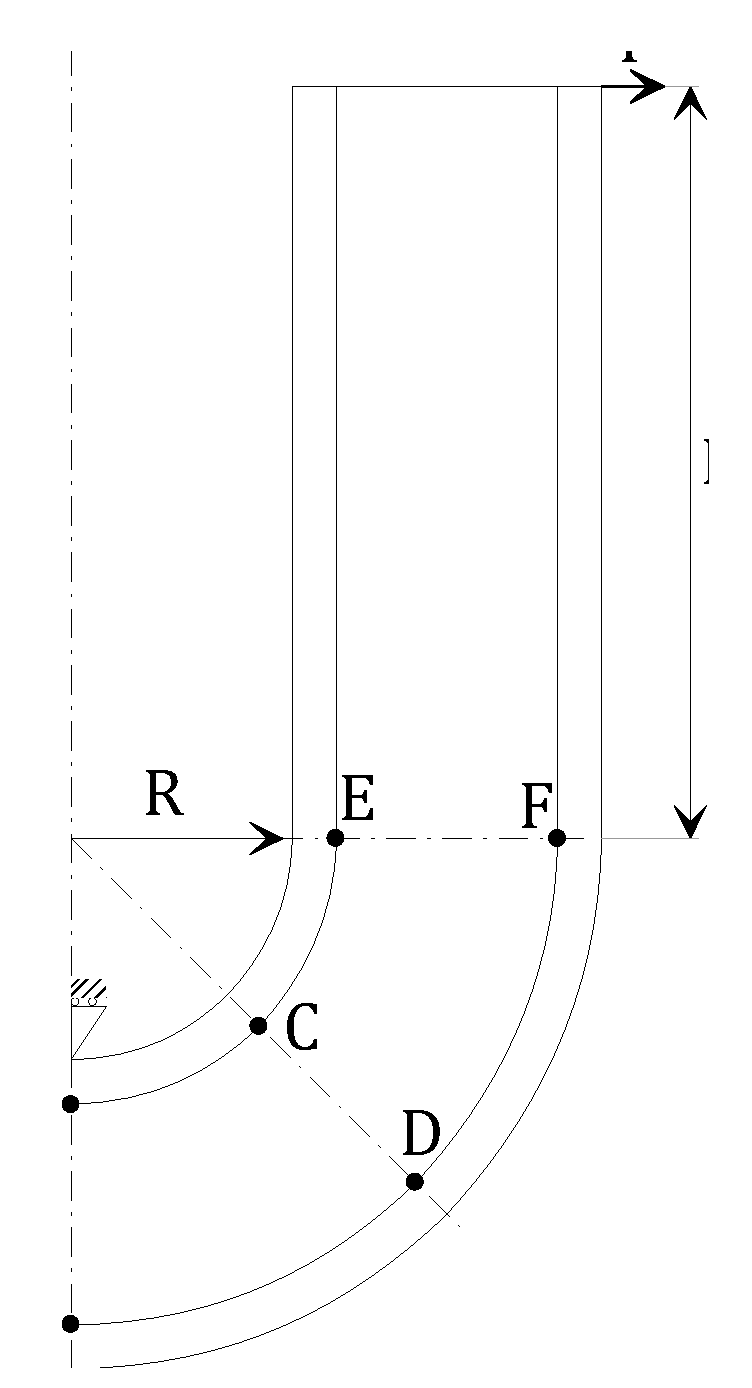
\includegraphics[height=80mm]{U-geo.eps} \hfill
  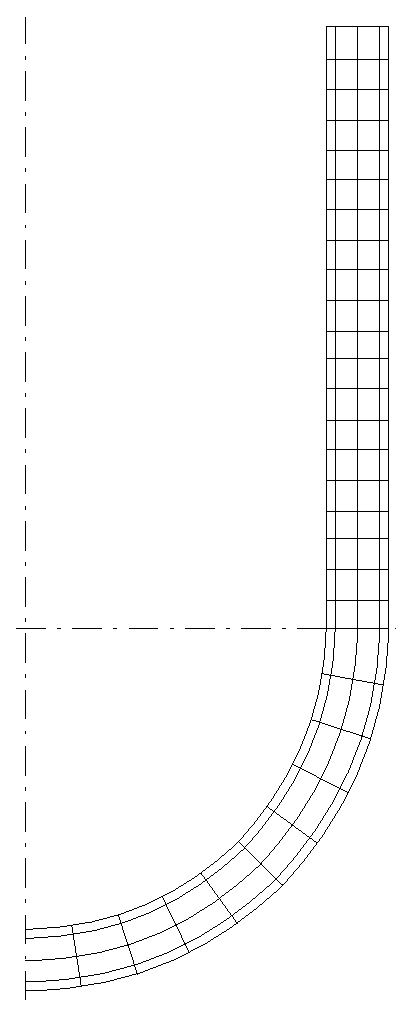
\includegraphics[height=80mm]{U-mesh1.eps}\hfill
  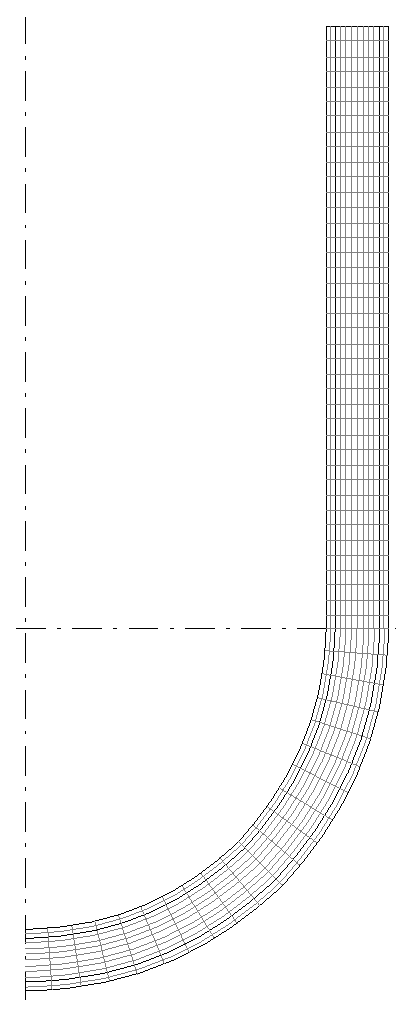
\includegraphics[height=80mm]{U-mesh2.eps}
  \caption{\label{Fig-poutU-geo} a) Géométrie de la poutre en U, b) le maillage utilisé pour le calcul (test de la méthode Reissner local,
c) maillage permettant d'obtenir la «solution de référence» puisqu'il n'y a pas de solution analytique}
\end{figure}

Disposant de la macro précédente, nous allons l'appliquer au calcul d'une poutre en~$U$.

Il s'agit d'une poutre sandwich dont les peaux sont en aluminium et l'âme en résine époxy. Par symétrie, seule une demi-poutre est modélisée. Elle est soumise à une force unitaire sur chaque montant.

\medskip
Les points pour lesquels nous nous intéresserons aux contraintes sont les points indiqués sur la \fig{Fig-poutU-geo}, à savoir les points A, B, C, D, E et F.



\medskip
Le listing \ansys est le suivant:

\color{gris}\scriptsize
\begin{multicols}{2}
\begin{Verbatim}[numbers=left,numbersep=3pt]
!* geom: partie droite
long=20
H1=0.2
H2=1.8
H3=2
!*
!* geom coude
Rint=10
Rh1=Rint+H1
Rh2=Rint+H2
Rh3=Rint+H3
!*
!* maillage
NCUTS=40
NRCUTS=20
NCORE=16
NSKIN=2
Forc=1
!*
/PREP7
!*
ET,1,PLANE82
!*
UIMP,1,EX, , ,70000,
UIMP,1,NUXY, , ,0.3,
UIMP,1,EMIS, , ,1,
!*
!*
UIMP,2,EX, , ,3400,
UIMP,2,NUXY, , ,0.34,
UIMP,2,EMIS, , ,1,
!*
k,1,0,-Rh3
k,2,Rh3,0
k,3,Rh2,0
k,4,0,-Rh2
k,5,0,-Rh1
k,6,Rh1,0
k,7,Rint,0
k,8,0,-Rint
k,9,Rh3,long
k,10,Rh2,long
k,11,Rh1,long
k,12,Rint,long
k,13,0,0
!*
larc,1,2,13,Rh3,NRCUTS
l,2,3,NSKIN
larc,4,3,13,Rh2,NRCUTS
l,1,4,NSKIN
l,4,5,NCORE
l,3,6,NCORE
larc,5,6,13,Rh1,NRCUTS
l,5,8,NSKIN
larc,8,7,13,Rint,NRCUTS
l,6,7,NSKIN
!*
l,2,9,NCUTS
l,9,10,NSKIN
l,10,3,NCUTS
l,10,11,NCORE
l,11,6,NCUTS
l,11,12,NSKIN
l,12,7,NCUTS
!*
mat,1
a,1,2,3,4
a,5,6,7,8
a,2,9,10,3
a,6,11,12,7
mat,2
a,4,3,6,5
a,3,10,11,6
mat,1
amesh,1
amesh,2
amesh,3
amesh,4
mat,2
amesh,5
amesh,6
!*
DL,4,,symm
DL,5,,symm
DL,8,,symm
!*
dk,8,uy,0
!*
fk,9,fx,Forc
!*
FINISH
/SOLU
/STAT,SOLU
SOLVE
FINISH
/POST1
pldisp,1
*USE,INTERF
...
\end{Verbatim}
\end{multicols}
\color{black}\normalsize

On utilise la macro en tapant \verb|*USE,INTERF|, et les contraintes sont directement modifiées dans \ansys. On peut alors utiliser les mêmes fonctions qu'habituellement pour visualiser les différentes composantes des contraintes.


\medskip
Le listing Cast3M est le suivant:

\color{gris}\scriptsize
\begin{multicols}{2}
\begin{Verbatim}[numbers=left,numbersep=3pt]
* geom: partie droite
long=20.0;
H1=0.2;
H2=1.8;
H3=2.0;
*
* geom coude
Rint=10.0;
Rh1=Rint+H1;
Rh2=Rint+H2;
Rh3=Rint+H3;
MRint = -1. * Rint;
MRh1 = -1. * Rh1;
MRh2 = -1. * Rh2;
MRh3 = -1. * Rh3;
*
* maillage
NCUTS=40;
NRCUTS=20;
NCORE=16;
NSKIN=2;
Forc=1.0;
*
OPTION DIMENSION 2 ELEMENT QUA4;
*
k1 = 0. MRh3;
k2 = Rh3 0.;
k3 = Rh2 0.;
k4 = 0. MRh2;
k5 = 0. MRh1;
k6 = Rh1 0.;
k7 = Rint 0.;
k8 = 0. MRint;
k9 = Rh3 long;
k10 = Rh2 long;
k11 = Rh1 long;
k12 = Rint long;
k13 = 0. 0.;
*
L1 = CERCLE NRCUTS k1 k13 k2 ;
L2 = DROITE k2 k3 NSKIN;
L3 = CERCLE NRCUTS k4 k13 k3 ;
L4 = DROITE k1 k4 NSKIN;
L5 = DROITE k4 k5 NCORE;
L6 = DROITE k3 k6 NCORE;
L7 = CERCLE NRCUTS k5 k13 k6 ;
L8 = DROITE k5 k8 NSKIN;
L9 = CERCLE NRCUTS k8 k13 k7 ;
L10 = DROITE k6 k7 NSKIN;
*
L11 = DROITE k2 k9 NCUTS;
L12 = DROITE k9 k10 NSKIN;
L13 = DROITE k10 k3 NCUTS;
L14 = DROITE k10 k11 NCORE;
L15 = DROITE k11 k6 NCUTS;
L16 = DROITE k11 k12 NSKIN;
L17 = DROITE k12 k7 NCUTS;
*
SURF1 = DALLER L1 L2 L3 L4;
SURF2 = DALLER L2 L11 L12 L13;
PEAUEXT = SURF1 ET SURF2;
* ELIMINE PEAUEXT;
SURF1 = DALLER L3 L6 L7 L5;
SURF2 = DALLER L6 L13 L14 L15;
AME = SURF1 ET SURF2;
* ELIMINE AME;
SURF1 = DALLER L8 L7 L10 L9;
SURF2 = DALLER L10 L15 L16 L17;
PEAUINT = SURF1 ET SURF2;
* ELIMINE PEAUINT;
PoutU = PEAUEXT ET AME ET PEAUINT;
*
Model1 = MODL peauext MECANIQUE ELASTIQUE ISOTROPE QUA4;
Model2 = MODL ame MECANIQUE ELASTIQUE ISOTROPE QUA4;
Model3 = MODL peauint MECANIQUE ELASTIQUE ISOTROPE QUA4;
ModelTot = Model1 ET Model2 ET Model3;
*
Mater1 = MATERIAU Model1 YOUNG 70000.0 NU 0.3 RHO 2700.0;
Mater2 = MATERIAU Model2 YOUNG 3400.0 NU 0.34 RHO 1000.0;
Mater3 = MATERIAU Model3 YOUNG 70000.0 NU 0.3 RHO 2700.0;
*
MR1 = RIGIDITE Model1 Mater1;
MR2 = RIGIDITE Model2 Mater2;
MR3 = RIGIDITE Model3 Mater3;
Mrigid = MR1 ET MR2 ET MR3;
*
CondL2 = BLOQUER UX (L4 ET L5 ET L8);
CondL1 = BLOQUER UY k8;
CondLtot = CondL1 ET CondL2;
FOR1 = FORCE(Forc 0.) k9;
Mrigid = Mrigid ET CondLtot;
*
Depl1 = RESOUD Mrigid For1 ;
*
UX1 = EXCO 'UX' depl1;
UY1 = EXCO 'UY' depl1;
Trace UX1 PoutU;
Trace UY1 PoutU;
*
def0 = DEFORMEE poutU Depl1 0.0 BLEU;
def1 = DEFORMEE poutU Depl1 ROUGE;
trace (def0 ET def1);
* ...
\end{Verbatim}
\end{multicols}
\color{black}\normalsize
Il reste maintenant à avoir les résultats dans les repères locaux élémentaires,
et voir ce qui se passe aux interfaces...




\medskip
\subsection{Résultats}

Dans les listings ci-dessus, nous n'avons pas exposé comme atteindre les contraintes, car cela sera fait en TP.

Les résultats directement obtenus sont donnés à la \fig{Fig-poutU-disp} pour la déformée et les déplacements selon~$x$ et~$y$, et à la \fig{Fig-poutU-eps} pour les déformations.
\begin{figure}[h!]
  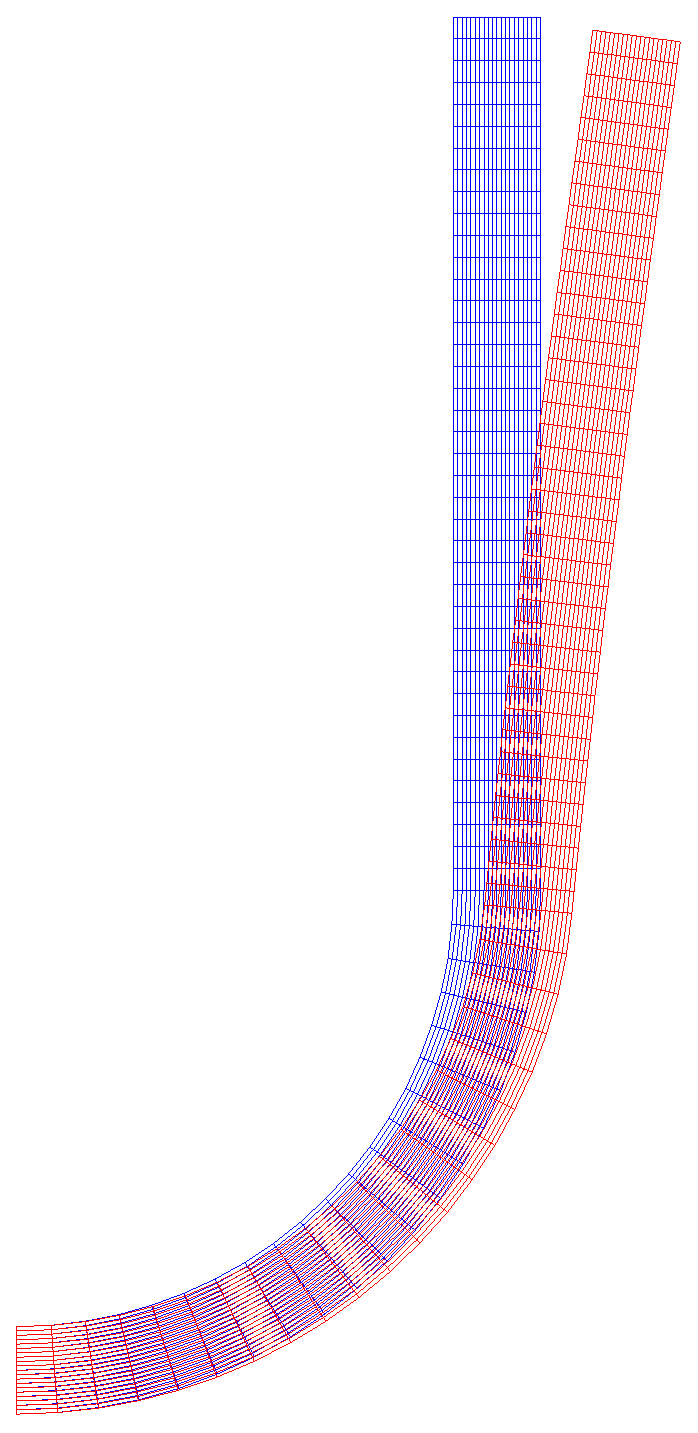
\includegraphics[height=80mm]{U-def.eps} \hfill
  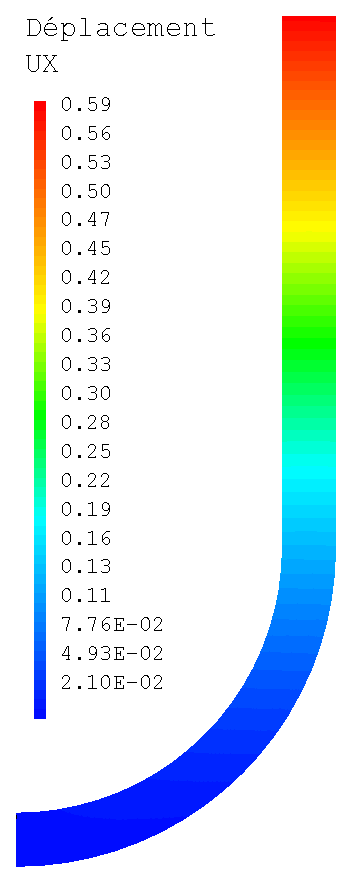
\includegraphics[height=80mm]{U-ux.eps}\hfill
  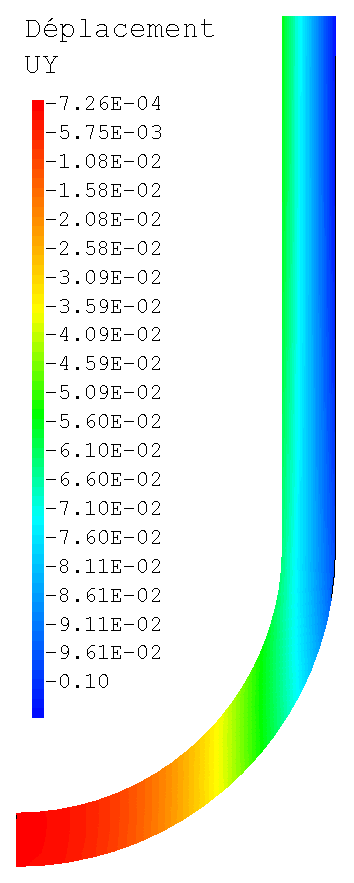
\includegraphics[height=80mm]{U-uy.eps}
  \caption{\label{Fig-poutU-disp} Déformée et déplacements}
\end{figure}
\begin{figure}[h!]
  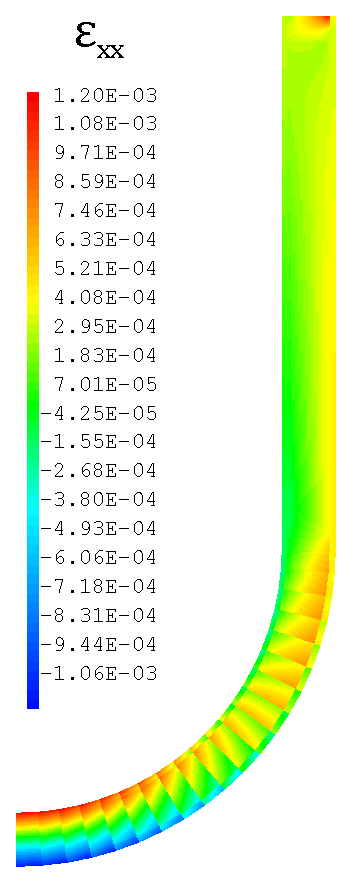
\includegraphics[height=80mm]{U-epsXX.eps} \hfill
  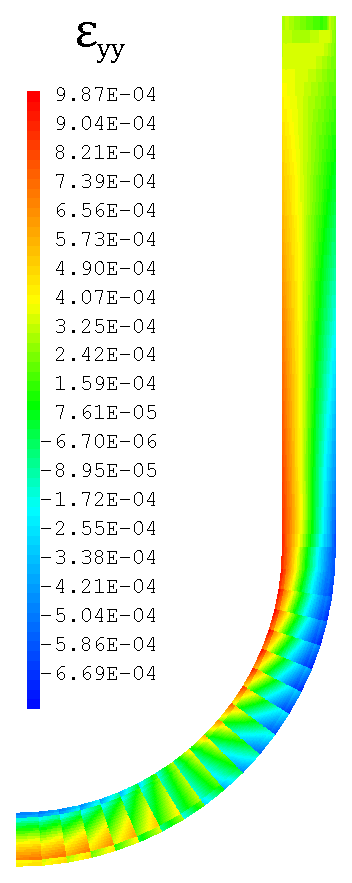
\includegraphics[height=80mm]{U-epsYY.eps}\hfill
  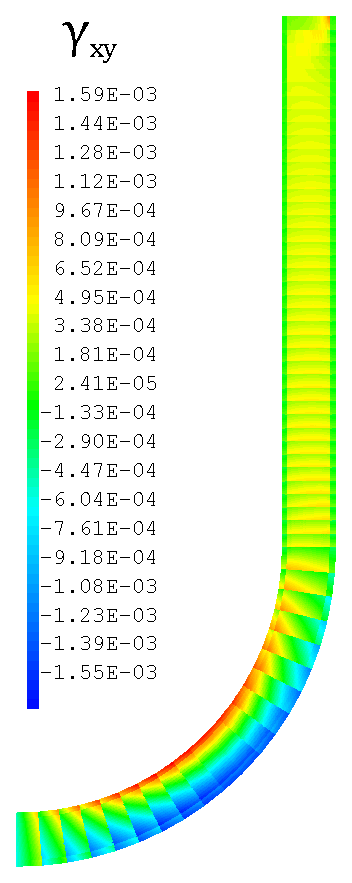
\includegraphics[height=80mm]{U-epsXY.eps}
  \caption{\label{Fig-poutU-eps} Déformations}\label{VMtiti}
\end{figure}

\medskip
Néanmoins nous présentons quelques résultats issus de l'analyse des contraintes aux interfaces avec ou sans utilisation de la méthode de Reissner local. Nous nous concentrerons sur les résultats numériques et graphiques permettant d'apprécier la précision de la méthode de Reissner local par rapport aux résultats d'\ansys aux points~$A$, $B$, $E$ et~$F$ ainsi que d'étudier l'influence de la valeur du rayon~$R$.

\medskip
Une première remarque s'impose: plus la valeur du rayon est faible, plus les résultats sont mauvais, quelle que soit la méthode employée (et vous devez savoir pourquoi à ce niveau du document).

\medskip
Au point~$A$, l'influence des conditions aux limites est encore sensible: en plus de la condition de symétrie de la structure, le blocage du déplacement vertical induit une légère détérioration des résultats numériques. L'influence de cette condition aux limites n'est plus visible au point~$B$.

\medskip
En~$A$ et~$B$, la composante discontinue est~$\sigma_{xx}$, les composantes~$\sigma_{yy}$ et~$\sigma_{xy}$ sont continues. Par contre, aux points~$E$ et~$F$, c'est~$\sigma_{yy}$ la composante discontinue et~$\sigma_{xx}$ et $\sigma_{xy}$ les composantes continues.
\newif\ifVMSurLaMemePage% Dernière fig et 1et tableau sur la même page si true
\VMSurLaMemePagetrue% vrai pour v2b cours

\medskip
D'après les résultats présentés ci-après, il est visible que la méthode de Reissner local permet d'améliorer les résultats par rapport à \ansys.
%
%
%\ifthenelse{\equal{1}{1}}{Même}{Différent}
%\newcounter{PageDeLImage}
%\setcounter{PageDeLImage}{\arabic{\pageref{VMtiti}}}
%\newboolean{VMSurLaMemePage}
%arabic \roman{\protect{\pageref{VMtiti}}} et \arabic{\pageref{VMtoto}};
%    \ifx&\arabic{\pageref{VMtiti}}&\arabic{\pageref{VMtoto}}%
%     true
%    \else
%     false!!!!
%    \fi
%\pageref{VMtiti},\pageref{VMtoto}%\unexpanded{\pageref{VMtiti}}
%\ifdef{\equal{1}{1}}{Même}{Différent}
%\ifthenelse{\equal{\pageref{VMtiti}}{\pageref{VMtoto}}}{True}{False}

%\ifthenelse{\equal{\expandafter{\pageref{Fig-poutU-eps}}}{\expandafter{\pageref{Tab:pt-A}}}}{Même}{Différent}
%\ifthenelse{\equal{\pageref{Fig-poutU-eps}}{\pageref{Tab:pt-A}}}{SUR LA MEME PAGE}{PAGES DIFFRENTES}
%\newpage


%\ifdef{\equal{\pageref{Fig-poutU-eps}}{\pageref{Tab:pt-A}}}{}{\clearpage}
\begin{table}[h!]\label{VMtoto}
\centering\small
  \begin{tabular}{|l||r|r|r|r|r|}
   \hline
   \multicolumn{1}{|c||}{\raisebox{-2.5mm}{Méthode}}&
   \multicolumn{1}{c}{\raisebox{-2.5mm}{$R$}}&
   \multicolumn{1}{|c}{$\sigma_{xx}$}&
   \multicolumn{1}{|c}{$\sigma_{xx}$}&
   \multicolumn{1}{|c}{\raisebox{-2.5mm}{$\sigma_{yy}$}}&
   \multicolumn{1}{|c|}{\raisebox{-2.5mm}{$\sigma_{xy}$}}\\[-3mm]
   &&
   \multicolumn{1}{|c}{peau}&
   \multicolumn{1}{|c|}{âme}&&\\
   &(mm)&
   \multicolumn{1}{|c}{(MPa)}&
   \multicolumn{1}{|c|}{(MPa)}&
   \multicolumn{1}{|c|}{(MPa)}&
   \multicolumn{1}{|c|}{(MPa)}\\
   \hline
   \hline
   Ref &10 &72,085 &4,0121 &1,5883 &-0,0023339  \\
   Reiss&10 &71,957 &3,9670 &1,5987 &-0,0155720  \\
   \ansys&10&71,957 &3,9670 & 1,5116 & 0,0086231  \\
   \hline
   Ref &8 &66,500 &3,8400 &1,8556 &-0,0022273  \\
   Reiss&8 &66,665 &3,7863 &1,8888 &-0,0118667  \\
   \ansys&8 &66,665 &3,7863 & 1,7943 & 0,0111910  \\
   \hline
   Ref &5 &57,289 &3,6598 &2,6317 &-0,0018770  \\
   Reiss&5 &57,727 &3,5771 &2,6979 &-0,0071024  \\
   \ansys&5 &57,727 &3,5771 & 2,6066 & 0,0128210  \\
   \hline
   Ref &3 &49,551 &3,6827 &3,9304 &-0,0014368  \\
   Reiss&3 &49,454 &3,5552 &4,0110 &-0,0046055  \\
   \ansys&3 &49,454 &3,5552 & 3,9621 & 0,0106410  \\
   \hline
   Ref &2 &42,699 &3,8289 &5,4227 &-0,0009727  \\
   Reiss&2 &42,362 &3,6593 &5,4785 &-0,0037443  \\
   \ansys&2 &42,362 &3,6593 & 5,5264 & 0,0059470  \\
   \hline
   Ref &1 &27,171 &4,3142 &9,2850 &-0,0004173  \\
   Reiss&1 &25,876 &4,0707 &9,1122 &-0,0021565  \\
   \ansys&1 &25,876 &4,0707 &9,6345 & 0,0005231  \\
   \hline
  \end{tabular}
\caption{\label{Tab:pt-A} Résultats au point~$A$}
\end{table}

%\begin{figure}
%\centering
%\input{tex/a-sxxc.2012.txt}
%
%  \caption{\label{Fig:asxxc}~$\sigma_{xx}$ dans l'âme en~$A$}
%\end{figure}
%
%\begin{figure}
%\centering
%\input{tex/a-sxxs.2012.txt}
%
%  \caption{\label{Fig:asxxs}~$\sigma_{xx}$ dans la peau en~$A$}
%\end{figure}

%\ifdef{\equal{\pageref{Fig-poutU-eps}}{\pageref{Tab:pt-A}}}{\clearpage}{}
\ifVMSurLaMemePage\clearpage\fi
\begin{figure}[h!]
\centering
\input{tex/a-syy.2012.txt}
\caption{\label{Fig:asyy}~$\sigma_{yy}$ en~$A$}
\end{figure}

%\ifdef{\equal{\pageref{Fig-poutU-eps}}{\pageref{Tab:pt-A}}}{}{\clearpage}
\ifVMSurLaMemePage\else\clearpage\fi
\begin{figure}[h!]
\centering
\input{tex/a-sxy.2012.txt}
\caption{\label{Fig:asxy}~$\sigma_{xy}$ en~$A$}
\end{figure}

%\ifdef{\equal{\pageref{Fig-poutU-eps}}{\pageref{Tab:pt-A}}}{\clearpage}{}%%%
\ifVMSurLaMemePage\clearpage\fi
\begin{table}[h!]
\centering\small
  \begin{tabular}{|l||r|c|c|c|c|}
   \hline
   \multicolumn{1}{|c||}{\raisebox{-2.5mm}{Méthode}}&
   \multicolumn{1}{c}{\raisebox{-2.5mm}{$R$}}&
   \multicolumn{1}{|c}{$\sigma_{xx}$}&
   \multicolumn{1}{|c}{$\sigma_{xx}$}&
   \multicolumn{1}{|c}{\raisebox{-2.5mm}{$\sigma_{yy}$}}&
   \multicolumn{1}{|c|}{\raisebox{-2.5mm}{$\sigma_{xy}$}}\\[-3mm]
   &&
   \multicolumn{1}{|c}{peau}&
   \multicolumn{1}{|c|}{âme}&&\\
   &(mm)&
   \multicolumn{1}{|c}{(MPa)}&
   \multicolumn{1}{|c|}{(MPa)}&
   \multicolumn{1}{|c|}{(MPa)}&
   \multicolumn{1}{|c|}{(MPa)}\\
   \hline
   \hline
   Ref& 10 & -72,248 & -3,0668 & 1,4080 & -0,0023570 \\
   Reiss&10 & -72,542 & -3,1193 & 1,2573 & -0,0138800 \\
   \ansys&10& -72,542 & -3,1193 & 1,5464 & -0,0198700 \\
   \hline
   Ref& 8 & -67,723 & -2,7905 & 1,5799 & -0,0026011 \\
   Reiss&8 & -68,001 & -2,8457 & 1,4570 & -0,0107700 \\
   \ansys&8 & -68,001 & -2,8457 & 1,7111 & -0,0197300 \\
   \hline
   Ref& 5 & -61,079 & -2,3199 & 2,0320 & -0,0024099 \\
   Reiss&5 & -61,335 & -2,3813 & 1,9460 & -0,0067001 \\
   \ansys&5 & -61,335 & -2,3813 & 2,1535 & -0,0186210 \\
   \hline
   Ref& 3 & -56,823 & -1,9080 & 2,6611 & -0,0022154 \\
   Reiss&3 & -57,072 & -1,9756 & 2,5888 & -0,0045050 \\
   \ansys&3 & -57,072 & -1,9756 & 2,7738 & -0,0176540 \\
   \hline
   Ref& 2 & -54,772 & -1,6200 & 3,2396 & -0,0021234 \\
   Reiss&2 & -55,026 & -1,6902 & 3,1612 & -0,0036124 \\
   \ansys&2 & -55,026 & -1,6902 & 3,3438 & -0,0172760 \\
   \hline
   Ref& 1 & -52,491 & -1,1687 & 4,2871 & -0,0020797 \\
   Reiss&1 & -52,777 & -1,2391 & 4,1625 & -0,0031088 \\
   \ansys&1 & -52,777 & -1,2391 & 4,3710 & -0,0174200 \\
   \hline
  \end{tabular}
  \caption{\label{Tab:pt-B} Résultats au point~$B$}
\end{table}
%\clearpage
%\begin{figure}
%\centering
%\input{tex/b-sxxc.2012.txt}
%
%  \caption{\label{Fig:bsxxc}~$\sigma_{xx}$ dans l'âme en~$B$}
%\end{figure}
%
%\begin{figure}
%\centering
%\input{tex/b-sxxs.2012.txt}
%
%  \caption{\label{Fig:bsxxs}~$\sigma_{xx}$ dans la peau en~$B$}
%\end{figure}
%

%\ifdef{\equal{\pageref{Fig-poutU-eps}}{\pageref{Tab:pt-A}}}{\clearpage}{}
\ifVMSurLaMemePage\else\clearpage\fi
\begin{figure}[h!]
\centering
\input{tex/b-syy.2012.txt}
\caption{\label{Fig:bsyy}~$\sigma_{yy}$ en~$B$}
\end{figure}

%\ifdef{\equal{\pageref{Fig-poutU-eps}}{\pageref{Tab:pt-A}}}{}{\clearpage}
\ifVMSurLaMemePage\clearpage\fi
\begin{figure}[h!]
\centering
\input{tex/b-sxy.2012.txt}
\caption{\label{Fig:bsxy}~$\sigma_{xy}$ en~$B$}
\end{figure}

%\ifdef{\equal{\pageref{Fig-poutU-eps}}{\pageref{Tab:pt-A}}}{\clearpage}{}
\ifVMSurLaMemePage\else\clearpage\fi
\begin{table}[h!]
\centering\small
  \begin{tabular}{|l||r|c|c|c|c|}
   \hline
   \multicolumn{1}{|c||}{\raisebox{-2.5mm}{Méthode}}&
   \multicolumn{1}{c}{\raisebox{-2.5mm}{$R$}}&
   \multicolumn{1}{|c}{$\sigma_{yy}$}&
   \multicolumn{1}{|c}{$\sigma_{yy}$}&
   \multicolumn{1}{|c}{\raisebox{-2.5mm}{$\sigma_{xx}$}}&
   \multicolumn{1}{|c|}{\raisebox{-2.5mm}{$\sigma_{xy}$}}\\[-3mm]
   &&
   \multicolumn{1}{|c}{peau}&
   \multicolumn{1}{|c|}{âme}&&\\
   &(mm)&
   \multicolumn{1}{|c}{(MPa)}&
   \multicolumn{1}{|c|}{(MPa)}&
   \multicolumn{1}{|c|}{(MPa)}&
   \multicolumn{1}{|c|}{(MPa)}\\
   \hline
   \hline
   ref& 10 &46,0340 &2,410200 &0,57548 &0,77518 \\
   Reiss&10 &46,0265 &2,397450 &0,48986 &0,71342 \\
   \ansys&10&46,0265 &2,397450 &0,62529 &0,80572 \\
   \hline
   ref& 8  &45,8625 &2,443000 &0,68465 &0,83563 \\
   Reiss&8 &45,8505 &2,421450 &0,62992 &0,76781 \\
   \ansys&8 &45,8505 &2,421450 &0,71910 &0,90760 \\
   \hline
   ref& 5  &45,4490 &2,539450 &1,00620 &1,00390 \\
   Reiss&5 &45,5025 &2,499550 &1,00810 &0,91559 \\
   \ansys&5 &45,5025 &2,499550 &0,94099 &1,19800 \\
   \hline
   ref& 3  &44,5760 &2,694400 &1,56820 &1,25790 \\
   Reiss&3 &45,0015 &2,644550 &1,62260 &1,10690 \\
   \ansys&3 &45,0015 &2,644550 &1,30760 &1,64980 \\
   \hline
   ref& 2  &43,1510 &2,856600 &2,23920 &1,50420 \\
   Reiss&2 &44,1375 &2,805000 &2,32600 &1,25870 \\
   \ansys&2 &44,1375 &2,805000 &1,77080 &2,12250 \\
   \hline
   ref& 1  &37,6330 &3,184100 &4,02110 &1,90380 \\
   Reiss&1 &40,1735 &3,143850 &4,04390 &1,41220 \\
   \ansys&1 &40,1735 &3,143850 &3,04360 &3,15350 \\
   \hline
  \end{tabular}
  \caption{\label{Tab:pt-E} Résultats au point~$E$}
\end{table}

%\begin{figure}
%\centering
%\input{tex/e-sxxc.2012.txt}
%
%  \caption{\label{Fig:esxxc}~$\sigma_{yy}$ dans l'âme en~$E$}
%\end{figure}
%
%\begin{figure}
%\centering
%\input{tex/e-sxxs.2012.txt}
%
%  \caption{\label{Fig:esxxs}~$\sigma_{yy}$ dans la peau en~$E$}
%\end{figure}
%
%\ifdef{\equal{\pageref{Fig-poutU-eps}}{\pageref{Tab:pt-A}}}{}{\clearpage}
\ifVMSurLaMemePage\clearpage\fi
\begin{figure}[h!]
\centering
\input{tex/e-syy.2012.txt}
\caption{\label{Fig:esyy}~$\sigma_{xx}$ en~$E$}
\end{figure}

%\ifdef{\equal{\pageref{Fig-poutU-eps}}{\pageref{Tab:pt-A}}}{\clearpage}{}
\ifVMSurLaMemePage\else\clearpage\fi
\begin{figure}[h!]
\centering
\input{tex/e-sxy.2012.txt}
\caption{\label{Fig:esxy}~$\sigma_{xy}$ en~$E$}
\end{figure}

%\ifdef{\equal{\pageref{Fig-poutU-eps}}{\pageref{Tab:pt-A}}}{}{\clearpage}
\ifVMSurLaMemePage\clearpage\fi
\begin{table}[h!]
\centering\small
  \begin{tabular}{|l||r|c|c|c|c|}
   \hline
   \multicolumn{1}{|c||}{\raisebox{-2.5mm}{Méthode}}&
   \multicolumn{1}{c}{\raisebox{-2.5mm}{$R$}}&
   \multicolumn{1}{|c}{$\sigma_{yy}$}&
   \multicolumn{1}{|c}{$\sigma_{yy}$}&
   \multicolumn{1}{|c}{\raisebox{-2.5mm}{$\sigma_{xx}$}}&
   \multicolumn{1}{|c|}{\raisebox{-2.5mm}{$\sigma_{xy}$}}\\[-3mm]
   &&
   \multicolumn{1}{|c}{peau}&
   \multicolumn{1}{|c|}{âme}&&\\
   &(mm)&
   \multicolumn{1}{|c}{(MPa)}&
   \multicolumn{1}{|c|}{(MPa)}&
   \multicolumn{1}{|c|}{(MPa)}&
   \multicolumn{1}{|c|}{(MPa)}\\
   \hline
   \hline
   ref & 10 & -47,438 &-2,1425 &0,54431 & 0,30073 \\
   Reiss&10 & -47,510 &-2,1533 &0,39416 & 0.38936 \\
   \ansys&10& -47,510 &-2,1533 &0,65814 & 0,30000 \\
   \hline
   ref & 8 & -47,4555 &-2,11415 &0,62480 & 0,24743 \\
   Reiss&8 & -47,5605 &-2,12825 &0,50447 & 0.33138 \\
   \ansys&8 & -47,5605 &-2,12825 &0,72921 & 0,21663 \\
   \hline
   ref & 5 & -47,415 &-2,03645 &0,83167 & 0,10558 \\
   Reiss&5 & -47,5335 &-2,05940 &0,76054 & 0,18360 \\
   \ansys&5 & -47,5335 &-2,05940 &0,87666 & 0,00251 \\
   \hline
   ref & 3 & -47,223 &-1,92305 &1,11940 &-0,10042 \\
   Reiss&3 & -47,1885 &-1,95170 &1,07760 &-0,01314 \\
   \ansys&3 & -47,1885 &-1,95170 &1,05090 &-0,28747 \\
   \hline
   ref & 2 & -46,940 &-1,81445 &1,38480 &-0,29901 \\
   Reiss&2 & -46,6760 &-1,84130 &1,35230 &-0,18934 \\
   \ansys&2 & -46,6760 &-1,84130 &1,21420 &-0,55238 \\
   \hline
   ref & 1 & -46,1935 &-1,61030 &1,85860 &-0,67358 \\
   Reiss&1 & -45,4620 &-1,62185 &1,81270 &-0,50497 \\
   \ansys&1 & -45,4620 &-1,62185 &1,52280 &-1,03400 \\
   \hline
  \end{tabular}
\caption{\label{Tab:pt-F} Résultats au point~$F$}
\end{table}

%\begin{figure}
%\centering
%\input{tex/f-sxxc.2012.txt}
%
%  \caption{\label{Fig:fsxxc}~$\sigma_{yy}$ dans l'âme en~$F$}
%\end{figure}
%
%\clearpage
%
%\begin{figure}
%\centering
%\input{tex/f-sxxs.2012.txt}
%
%  \caption{\label{Fig:fsxxs}~$\sigma_{yy}$ dans la peau en~$F$}
%\end{figure}

%\ifdef{\equal{\pageref{Fig-poutU-eps}}{\pageref{Tab:pt-A}}}{\clearpage}{}
\ifVMSurLaMemePage\else\clearpage\fi
\begin{figure}[h!]
\centering
\input{tex/f-syy.2012.txt}
\caption{\label{Fig:fsyy}~$\sigma_{xx}$ en~$F$}
\end{figure}

%\ifdef{\equal{\pageref{Fig-poutU-eps}}{\pageref{Tab:pt-A}}}{}{\clearpage}
\ifVMSurLaMemePage\clearpage\fi
\begin{figure}[h!]
\centering
\input{tex/f-sxy.2012.txt}
\caption{\label{Fig:fsxy}~$\sigma_{xy}$ en~$F$}
\end{figure}
%\clearpage
% macro Ansys et poutre en U
\fi


\medskip
\section{Sous-structuration et simulation multi-échelles}\label{Sec-ssstruc}\index{Sous-structuration}\index{Multi-échelles}

Le fonctionnement des produits industriels met en jeu des phénomènes physiques à des
échelles très différentes.
La prise en compte de tous ces phénomènes dans les simulations numériques demanderait
d'utiliser des modèles extrêmement détaillés, entraînant des coûts d'identification
et/ou de calcul prohibitifs.
La simulation multi-échelles\index{Multi-échelles} est une réponse à cette problématique.
Elle consiste à simuler chaque phénomène à l'échelle la plus pertinente,
i.e. en utilisant plusieurs modèles de tailles et de finesses différentes; cela permet,
grâce à des solveurs adaptés, de réaliser des simulations qui seraient inaccessibles
par des approches plus directes.

\medskip
Imaginons que nous souhaitions calculer un avion, mais que, pour des raisons
évidente de sécurité nous ayons besoin d'obtenir une precision <<~boulon par boulon~>>.
On se doute bien que l'on ne peut mailler tout l'avion avec un tel niveau de détail...
On recourt alors à une cascade de modèles de dimensions et de finesses différentes,
allant de l'avion tout entier (mais modélisé relativement grossièrement) à
des détails structuraux modélisés très finement (mais limités à de petites zones), comme
montré sur la \fig{Fig-avion}.
\begin{figure}[ht]
\centering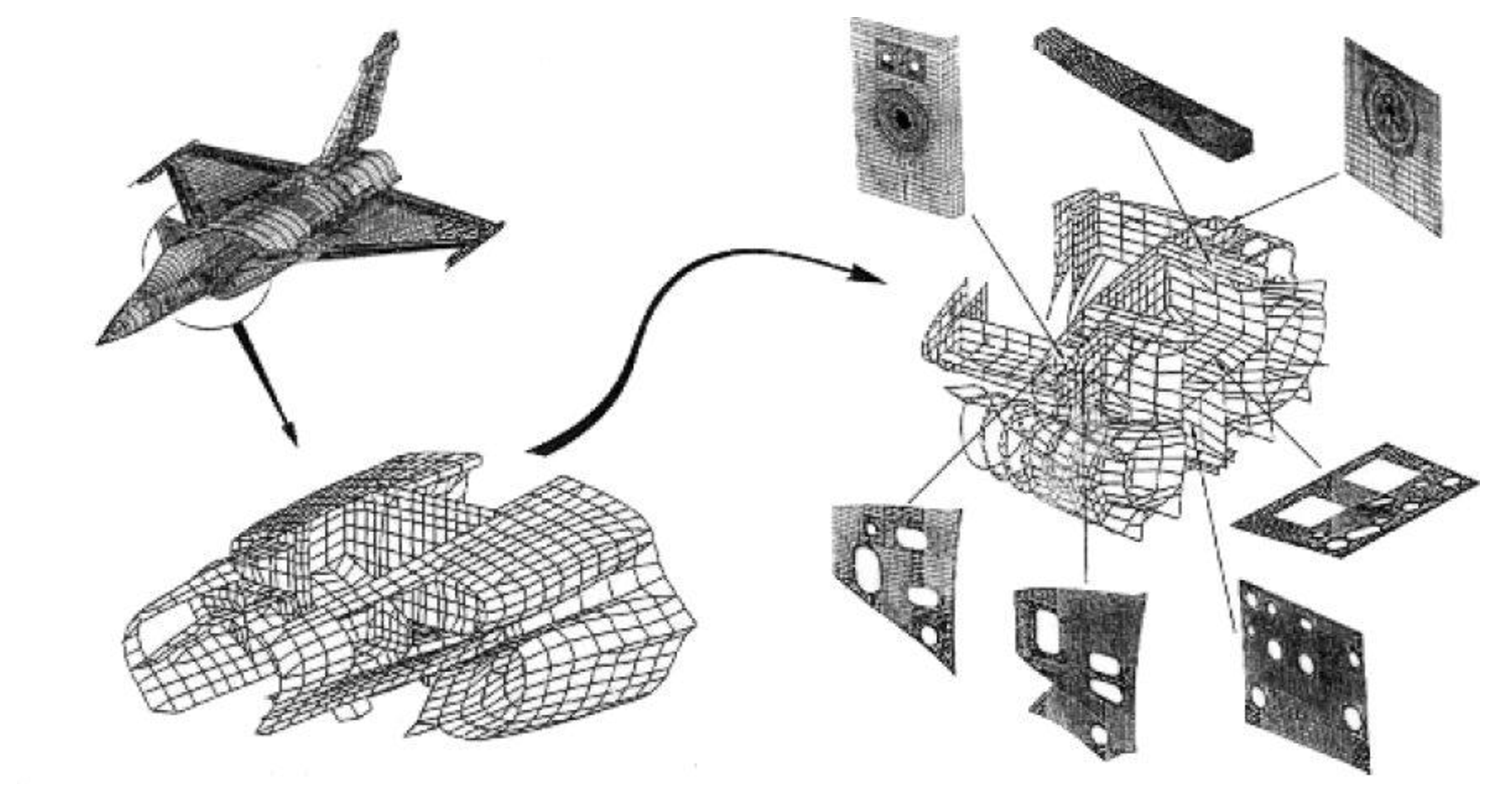
\includegraphics[height=60mm]{avion.eps}
\caption{Sous-structuration en aéronautique}\label{Fig-avion}
\end{figure}

La simulation est donc décomposée en différents niveaux, chacun représentant une échelle
différente. Pour coordonner ces niveaux entre eux, on utilise généralement une
\textcolorblue{approche} dite \textcolorblue{descendante}:\index{Approche descendante}
on commence par simuler  le comportement global de l'avion, puis les résultats sont utilisés pour
déterminer les conditions aux limites appliquées sur les niveaux inférieurs.
Toutefois, il est parfois également nécessaire de combiner ces approches descendantes
à des \textcolorblue{approches ascendantes}:\index{Approche ascendante}
les résultats des simulations fines sont utilisés pour construire des modèles de comportements
plus grossiers.

\medskip
De très nombreuses méthodologies multi-échelles existent et reposent
toutes sur le fait de simuler chaque phénomène à l'échelle la plus
pertinente.
Pour cela, il est nécessaire:
\begin{enumerate}
   \item de \textcolorred{distinguer différentes échelles} dans la modélisation et dans la simulation;
   \item de \textcolorred{modéliser les relations existant} entre ces différentes échelles.
\end{enumerate}

\medskip
Considérons un problème comportant deux échelles.
Le point 1 évoqué ci-dessus se traduit par le fait de disposer de deux modèles
distincts:
\begin{itemize}
   \item \textcolorblue{Un modèle macroscopique}\index{Modèle macroscopique}

	Il représente le produit et son environnement extérieur et est constitué
	d'une géométrie et d'un modèle de comportement relativement grossiers
	(puisque n'ayant pas vocation à représenter les phénomènes microscopiques);
   \item \textcolorblue{Un modèle microscopique}\index{Modèle microscopique}

	Il possède une description géométrique et un maillage suffisamment fins ainsi qu'un
	modèle de comportement détaillé. Il ne comprend qu'une ou quelques
	<<~cellules types~>> de petites dimensions.

	Il est souvent possible, pour les matériaux notamment, de disposer d'hypothèses
	simplificatrices (telles que l'élasticité linéaire) permettant de se restreindre à une
	seule cellule type.
	Pour le cas des matériaux anisotropes constitués de plusieurs autres matériaux tels
	que les matériaux composites et fibreux, on se reportera au chapitre suivant sur l'homogénéisation.

	Toutefois, certaines fois on ne dispose pas de telles hypothèses et il faut multiplier le nombre
	de cellules (jusqu'à parfois couvrir tout le modèle macro !)
\end{itemize}

\medskip
Le point 2 consiste donc à relier les deux échelles de modélisation.

En effet, les modèles macro et micro ne sont pas indépendants puisqu'ils
modélisent la même physique à des échelles différentes.
Il est donc nécessaire qu'ils soient cohérents l'un vis-à-vis de l'autre, en tout point et à
chaque instant de la simulation.
Pour cette raison, les modélisations multi-échelles\index{Multi-échelles} comportent des couplages, i.e. des
modèles d'interactions, entre les échelles.

Dans le cadre de la mécanique des solides déformables, on procède
généralement comme suit:
\begin{itemize}
   \item Le modèle de comportement macroscopique:\index{Modèle macroscopique}
	qui modélise des phénomènes se produisant <<~au cœur du matériau~>>,
	doit correspondre à la relation contraintes/déformations observée sur la cellule micro ;

   \item Le modèle de comportement microscopique:\index{Modèle microscopique}
	qui traduisent la façon dont la cellule est sollicitée par son environnement
 	extérieur, doivent correspondre à l'état de contraintes ou de déformations macro.
\end{itemize}

Le modèle macro ayant une résolution beaucoup plus grossière, la cohérence des deux
modèles ne peut donc pas se traduire par une correspondance exacte, point par point, des
conditions aux limites ou du comportement. Pour cette raison, la plupart des approches
multi-échelles postulent que les quantités macroscopiques doivent correspondre à des
<<~moyennes~>> des quantités micro correspondantes,  la définition mathématique exacte de
cette moyenne variant fortement d'une approche à l'autre.

\medskip
\colorgreen On peut donc dire que:
\begin{itemize}
   \item Le modèle de comportement macroscopique\index{Modèle macroscopique} d'un élément de volume est choisi
	égal au comportement moyen de la cellule micro correspondante, calculé en utilisant
	une technique d'homogénéisation;\index{Homogénéisation}

   \item Les conditions aux limites micro sont appliquées en moyenne, car les champs de
	contraintes ou de déplacements macro sont beaucoup trop grossiers.
\end{itemize}\colorblack

\medskip
Le problème est donc \textcolorred{d'échanger des données pertinentes entre les
différentes échelles}, compte tenu des différentes résolutions des modèles.

\medskip
\textcolorred{Dans le sens micro vers macro, on utilisera les techniques d'homogénéisation} \index{Homogénéisation}
dont il sera l'objet au chapitre suivant.

\medskip
\textcolorred{Dans le sens macro vers micro, il s'agit donc de spécifier des conditions aux limites
à appliquer sur le bord des cellules micro, à partir d'une solution macro.}

\textcolorgris{%
Les méthodes les plus simples se contentent d'imposer directement le champ de déplacements (ou
de contraintes) macro comme condition aux limites. Le modèle macro ayant par définition une
résolution beaucoup plus grossière que le modèle micro, il  est incapable de capturer l'allure
microscopique des déplacements ou des contraintes. Ces CL sont donc souvent trop imprécises
par rapport aux finalités du modèle micro. Cela peut dégrader fortement la qualité des
résultats et donc restreindre le domaine de validité de ces approches.%
}

Pour palier ce problème, on écrit les CL micro de manière plus subtile en les décomposant
en la somme d'un terme moyen et d'un terme de moyenne nulle. Ainsi, le champ micro $u^m$
sera écrit $u^m=u^M +v^m$ où $u^M$ est le champ macro (i.e. la moyenne  du champ micro),
et $v^m$ est le reste (à moyenne nulle).
Notre problème devient donc de \textcolorred{déterminer le reste $v^m$}, et c'est là
que les méthodes divergent le plus. On distingue néanmoins deux grosses familles:
\begin{itemize}
   \item \textcolorblue{Condition de périodicité}\index{Condition de périodicité}

	On postule que l'on connaît l'allure du reste. On peut alors enchaîner un calcul macro
	avec un solveur spécifique puis un calcul micro avec un solveur classique;
   \item \textcolorblue{Couplage des cellules micro}\index{Couplage des cellules micro}

	Lorsqu'il n'est pas si simple de <<~séparer~>> les échelles, alors il faut résoudre
	en même temps les deux problèmes micro et macro avec échange de données.
\end{itemize}
Ces deux approches vont être un peu plus détaillées maintenant.




\medskip
\subsection{Condition de périodicité -- méthodes multi-niveaux}\index{Condition de périodicité}\index{Multi-niveaux}

Souvent, les méthodes multi-niveaux sont basées sur des conditions de périodicité
inspirées de l'homogénéisation périodique.\index{Homogénéisation}
Ces conditions supposent que la partie micro du champ de déplacement, $v^m$, est périodique,
i.e. est égale sur chaque paire de faces opposées de la cellule type considérée.
La même hypothèse est formulée sur les contraintes.
On obtient ainsi un ensemble de CL permettant de déterminer entièrement la solution micro à
partir d'une déformation (ou d'une contrainte) macro imposée.

Le résultat micro ainsi obtenu est pertinent à deux conditions:
1) il faut que la microstructure soit effectivement périodique, et 2) que le principe de
Saint-Venant\index[aut]{Saint-Venant (Adhémar Jean Claude Barré de -), 1797-1886, Français}\index{Principe de Saint-Venant}
s'applique, i.e. que l'on se trouve suffisamment loin de la surface de la pièce
(y compris des détails géométriques tels que des trous, des fissures...).
Dans le cas contraire, des effets de bord peuvent affecter l'allure de la solution, qui n'est
alors plus périodique: il faut donc recourir à d'autres modélisations.

\medskip
La simulation multi-niveaux\index{Multi-niveaux} fait appel à deux types de modèles, chacun équipé de son solveur:
\begin{itemize}
   \item un modèle macro\index{Modèle macroscopique} ne possédant pas de relation de comportement du matériau
	prédéfinie, équipé d'un solveur EF modifié;
   \item un ensemble de modèles micro\index{Modèle microscopique} ne possédant pas de CL prédéfinies,
	équipés de solveurs EF classiques.
\end{itemize}

En fait, le solveur EF modifié est un solveur EF classique avec une petite différence:
à chaque fois que le solveur macro a besoin du comportement d'un élément de volume
quelconque, il envoie l'état de déformation macro de cet élément au solveur micro.
Ce dernier a alors toutes les données nécessaires pour simuler numériquement son comportement
à l'échelle microscopique. Il renvoie alors l'état de contraintes macro, selon la décomposition
mentionnée ci-dessus.
\textcolorgreen{Les cellules micro étant pour ainsi dire <<~indépendantes~>>, il est possible de
recourir à des calculateur parallèles.}

Le domaine de validité de ces méthodes est bon dès que l'on sait faire des hypothèses
réalistes sur l'allure de la solution micro. Ce n'est pas toujours le cas: par exemple, la fissuration,
lorsqu'elle sort d'un cadre microscopique pour atteindre un cadre macroscopique, se prête
très mal à cet exercice.
Le cas de la fissuration sera traitée dans un chapitre ultérieur de ce document.

\medskip\colorgreen
\textbf{En résumé:}

Les méthodes multi-niveaux abordent la simulation à l'échelle macro\index{Modèle macroscopique}
et se <<~nourrissent~>>  du comportement simulé à l'échelle microscopique.\index{Modèle microscopique}

Dans les méthodes multi-niveaux,\index{Multi-niveaux} l'emploi d'hypothèses de périodicité se traduit par
des <<~sauts~>> de contraintes et de déplacements d'une cellule à l'autre; si les échelles sont
mal séparées, ces sauts sont non négligeables. Ne correspondant à priori pas à la physique,
ils traduisent un écart avec la réalité.
\colorblack



\medskip
\subsection{Couplage des cellules micro -- méthodes de décomposition de domaine}\index{Couplage des cellules micro}\index{Décomposition de domaine}\label{Sec-dec}

Les méthodes multi-niveaux présentées au paragraphe précédent sont mises à mal
lorsque le comportement micro <<~déborde~>> un peu sur le comportement macro, i.e.
lorsque les échelles ne sont pas suffisamment bien séparées.
On recourt alors aux méthodes de décomposition de domaines,\index{Décomposition de domaine}
dont la validité est plus large, mais qui sont plus complexes.

\medskip
Puisque nous ne pouvons plus supposer une allure de la solution micro,\index{Modèle microscopique}
nous n'allons utiliser que les seules connaissance disponibles à priori: la continuité du champ de déplacements
ainsi que la vérification par les contraintes du principe d'action-réaction. Il <<~suffit~>> donc
d'écrire qu'à l'interface entre deux cellules micro, il y a égalité des déplacements et
nullité de la somme des traces\index{Trace} des contraintes (on retrouve ce que nous avons déjà
plusieurs fois évoqué avec l'état des contrainte à l'interface entre deux matériaux
différents).

\medskip
La présence de couplages entre les cellules micro\index{Couplage des cellules micro}
(qui en quelque sorte correspond à une généralisation de la condition de périodicité
du paragraphe précédent) change complètement le déroulement de la simulation par
rapport aux méthodes  multi-niveaux vues au paragraphe précédent.
En effet, la prise en compte de ces couplages implique d'échanger directement des données
entre les différents solveurs micro, qui ne sont plus <<~indépendants~>>.
En contrepartie, cela permet de propager une information fine sur l'ensemble de la pièce et,
ainsi, de se passer de l'hypothèse de séparation des échelles: il n'est plus nécessaire de
modéliser séparément les phénomènes micro et macro.

\medskip
Concrètement, les méthodes de décomposition de domaine\index{Décomposition de domaine}
sont des solveurs, qui ont généralement un fonctionnement multi-échelles.\index{Multi-échelles}
Elles partent d'un modèle micro\index{Modèle microscopique} du produit
décomposé en sous-structures, et consistent à coupler les sous-structures en échangeant des
contraintes et des déplacements sur les interfaces.
Des versions plus ou moins simples existent. Notons bien qu'il n'y a pas de modèle macro
dans une telle approche.

\medskip\colorgreen
\textbf{En résumé:}

Dans la décomposition de domaine,\index{Décomposition de domaine} la simulation est abordée
à l'échelle la plus fine: la sous-structuration et le problème grossier ne sont utilisés que pour
améliorer l'efficacité de la résolution.

Une simulation par décomposition de domaine\index{Décomposition de domaine} conduit toujours
à un champ de déplacement micro continu sur toute la structure, et un champ de contraintes micro
équilibré (au sens des EF) sur toute la structure.
\colorblack

\medskip
\textcolorgris{Actuellement, la simulation multi-échelles\index{Multi-échelles} est encore
relativement peu répandue dans le monde de l'ingénierie. Elle représente en effet un changement
considérable par rapport aux pratiques usuelles de simulation; de plus, la plupart des logiciels de
calcul multi-échelles\index{Multi-échelles} sont des outils développés par des chercheurs, qui
n'ont pas encore l'ergonomie et la robustesse des solveurs utilisés dans l'industrie. Les industriels
attendent donc l'apparition d'outils mieux adaptés à leurs problématiques avant d'envisager
une utilisation plus fréquente de ces méthodes.}

\textcolorgris{Cependant, à plus long terme, la simulation multi-échelles\index{Multi-échelles}
suscite un intérêt considérable dans l'industrie: en rendant accessibles à la simulation
des phénomènes qui ne peuvent actuellement être étudiés qu'expérimentalement,
elle constitue un pas important en direction du <<~virtual testing~>>.
Pour cette raison, elle fait toujours l'objet de nombreux projets de recherche.
Ceux-ci concernent aussi bien la modélisation, avec notamment la mise au point de
<<~matériaux virtuels~>> (qui ne sont rien d'autre que des modèles multi-échelles, notamment
pour les matériaux composites), que les solveurs qui sont en constante évolution.}

\medskip
\section{Super-éléments}\index{Super-élément}

Dans ce paragraphe, nous allons parler du concept de super-élément, qui n'est qu'une
application de ce qui a été présenté au paragraphe précédent.

\medskip
Un super-élément\index{Super-élément} est un groupement d'éléments qui, après
assemblage, peuvent être vus comme un élément individuel du point de vue du calcul.
Cet assemblage peut être requis pour des raisons de modélisation ou de calcul.

Pour constituer un super-éléments,\index{Super-élément} les éléments groupés ne peuvent être
pris au hasard. Ils doivent au moins constituer une <<~structure~>> en eux-même, mais
d'autres conditions sont nécessaires qui seront détaillées plus loin.

Comme nous l'avons dit au paragraphe précédent, il y a deux voies duales pour considérer
ce processus.

L'approche descendante consiste à considérer un super-élément comme constitué
d'un ensemble d'éléments. On parle alors de macro-élément.\index{Macro-élément}
L'approche ascendante consiste à considérer un super-élément comme un sous-ensemble
d'une structure complète. On parle alors de sous-structure.\index{Sous-structure}\index{Sous-structuration}

Finalement, quand parle-t-on de sous-structure ou de macro-élément?\index{Macro-élément}\index{Sous-structure}\index{Sous-structuration}
En fait, il n'y a pas de règle, et le terme générique de super-élément couvre tout le
spectre depuis l'élément individuel jusqu'à la structure complète.

\medskip
\begin{histoire}
Originellement introduit dans l'aéronautique dans les années 60 (d'où le schéma
au paragraphe précédent), le concept de sous-structuration\index{Sous-structuration}
répondait à trois motivations:
\begin{itemize}
   \item faciliter la division du travail:
	des sous-structures\index{Sous-structure} avec des fonctions différentes (fuselage, ailes, train d'atterrissage...)
	pouvaient être traitées par des groupes d'experts différents. Chaque groupe pouvait
	à loisir améliorer, raffiner... sa partie tant que l'interface avec les autres parties
	restait inchangée.
   \item profiter de la répétition:
	en remarquant qu'une même structure peut contenir plusieurs sous-structures identiques,
	il est possible de diminuer le temps d'étude (par exemple symétrie des ailes...)
   \item contourner les limitations des ordinateurs:
	les ordinateurs de l'époque atteignaient vite leurs limites (par exemple en terme
	de taille mémoire). Diviser une structure complexe, que l'on était incapable de
	calculer en une seule fois, permettait de sauvegarder des résultats sous-structure
	par sous-structure puis d'effectuer <<~l'assemblage~>> des résultats.
\end{itemize}
Si les deux premiers points sont toujours d'actualité, le troisième l'est moins, surtout
depuis le recourt aux algorithmes parallèles.

C'est d'ailleurs le développement  de procédures pour le calcul parallèle qui a conduit
les mathématiciens appliqués au concept de sous-domaines, alors qu'ils devaient grouper
des éléments pour des raisons de calcul.
\end{histoire}
\colorblack

\medskip
\subsection{Condensation statique}\index{Condensation statique}\label{Sec-condens}

En tant qu'assemblage de plusieurs éléments, un super-élément\index{Super-élément} possède:
\begin{itemize}
   \item des degrés de liberté internes:
	qui ne sont pas connectés à des éléments n'appartenant pas au super-élément considéré.
	Les nœuds ayant des ddl internes sont dits nœuds internes.
   \item des degrés de liberté aux frontières:
	qui sont connectés à au moins une entité (élément, super-élément)
	n'appartenant pas au super-élément considéré.
\end{itemize}

L'opération consistant à éliminer tous les ddl internes est appelée
\textcolorblue{condensation statique} ou \textcolorblue{condensation}.\index{Condensation statique}
\medskip
Regardons ce qui se passe d'un point de vue matriciel.
Pour cela, considérons que nous ayons à résoudre le système:
\begin{equation}  \MM{K} \VV{q}=\VV{f}\end{equation}
Le vecteur $\VV{q}$ se compose des composantes internes $\VV{q_i}$ et des composantes
de frontière $\VV{q_b}$, de sorte que le système, une fois réordonné s'écrit:
\begin{equation}
\begin{bmatrix}
\mathbf{K_{bb}} & \mathbf{K_{bi}}\\
\mathbf{K_{ib}} & \mathbf{K_{ii}}
\end{bmatrix}
\begin{pmatrix}
\mathbf{q_b}\\\mathbf{q_i}
\end{pmatrix}
=
\begin{pmatrix}
\mathbf{f_b}\\\mathbf{f_i}
\end{pmatrix}
\end{equation}
Si la matrice $\MM{K}_{ii}$ n'est pas singulière, alors la seconde équation peut être
résolue en terme de variables internes en:
\begin{equation}
\VV{q_i} = \MMI{K_{ii}}\left(\VV{f_i}-\MM{K_{ib}}\VV{q_b}\right)
\end{equation}
En reportant cela dans la première équation, on obtient le système avec \textcolorblue{matrice
de rigidité condensée}:\index{Condensation statique}
\begin{equation}
\MM{\tilde{K}_{bb}}\VV{q_b} = \VV{\tilde{f}_b}
\end{equation}
avec:
\begin{equation}
\MM{\tilde{K}_{bb}}=\MM{K_{bb}} - \MM{K_{bi}}\MMI{K_{ii}}\MM{K_{ib}}
\quad \text{ et }\quad
\VV{\tilde{f}_b}=\VV{f_b} - \MM{K_{bi}}\MMI{K_{ii}}\VV{f_i}
\end{equation}
Après condensation, on peut donc bien considérer le super-élément, d'un point de vue calculatoire,
comme un élément individuel.

\medskip
Notons que la matrice $\MM{K_{ii}}$ n'est pas singulière si elle possède la \textcolorblue{condition
de rang suffisant}, i.e. si elle ne contient que des modes à énergie nulle correspondant aux
modes rigides (cette condition a déjà évoquée à propos de la validation des éléments).
Si cela n'est pas le cas, le super-élément\index{Super-élément} est dit \textcolorblue{flottant}, et
peut quand même être traité (en utilisant les projecteurs et inverses généralisés,
mais c'est un peu plus compliqué).

La condensation statique\index{Condensation statique} est une opération matricielle
appelée \textcolorblue{inversion partielle} ou \textcolorblue{élimination partielle} ou
\textcolorblue{pseudo-inversion}.\index{Pseudo-inversion}

\medskip
\subsection{Remonter aux ddl internes}
Une fois le système condensé résolu, on obtient les valeurs aux nœuds
internes en réutilisant la formule:
\begin{equation}
\VV{q_i} = \MMI{K_{ii}}\left(\VV{f_i}-\MM{K_{ib}}\VV{q_b}\right)
\end{equation}

\medskip
\section{Pseudo-inversion et réanalyse}\index{Pseudo-inversion}\label{Sec-PInv}
\textcolorgreen{On peut être amené, notamment lors de phases de conceptions, à devoir considérer plusieurs
problèmes <<~relativement proches~>> les uns des autres (i.e. tester plusieurs configurations).
On est alors tenté d'utiliser tout ou partie de la première modélisation afin de
réaliser les suivantes.}

\medskip
L'idée de la méthode de réanalyse est d'analyser le comportement d'une structure
élastique par EF \textcolorblue{sans particulariser} le système d'équations final par la prise en
compte de conditions cinématiques.

On obtient alors une solution générale de ce système faisant intervenir une
\textcolorblue{matrice de rigidité régularisée}. La nature de cette matrice (somme
d'une matrice bande et d'une matrice pleine) ne permet pas d'utiliser les méthodes
les plus classiques et optimales de résolution, mais il est possible d'en développer d'autres
permettant d'accéder à \textcolorblue{la quasi-inverse d'une matrice singulière semi-définie
positive} (tout en profitant de son caractère bande).\index{Pseudo-inversion}

Il est alors possible, tout en modifiant les conditions cinématiques et les chargements appliqués,
de procéder à des réanalyses qui consistent alors simplement à résoudre des systèmes
dits secondaires de tailles très inférieures au système global (mais un surcoût a été
<<~payé~>> initialement pour calculer la pseudo-inverse).

Des problèmes de contact avec ou sans frottement entre solides élastiques peuvent
bénéficier de cette méthode, ainsi que la modélisation du comportement élastique
incompressible.

\medskip
\textcolorred{Dans ce paragraphe sur la réanalyse, nous n'utiliserons pas la notation avec les
crochets et les accolades pour les matrices et les vecteurs afin d'alléger l'écriture}.


\medskip
\subsection{Modification du chargement uniquement}
Restons sur le problème structurel correspondant au système matriciel:
%une structure, de matrice de rigidité $\MM{K}$, alors les déplacements de ses
%nœuds $q$, lorsque cette structure est soumise au chargement $F$ sont donnés par
%le système:
\begin{equation}
\MM{K} \VV{q} = \VV{f}
\end{equation}
où $\MM{K}$ est de dimension $n\times n$.%, et $\VV{q}$ et $\VV{f}$ sont des vecteurs \textcolorgris{(on ne
%note plus $[K]\{q\}=\{F\}$ dans ce paragraphe)}.

\medskip
Si l'on souhaite considérer plusieurs cas de chargement $\VV{F_1},\ldots,\VV{F_k}$, on peut soit résoudre
$k$ fois le système précédent, soit résoudre le système:
\begin{equation}
\MM{K} \MM{\overline{q}} =\MM{\overline{F}}
\end{equation}
où $\MM{\overline{F}}$ est la matrice $n\times k$ des $k$ vecteurs de chargement, et $\MM{\overline{q}}$ est la
matrice $n\times k$ des $k$ vecteurs solutions correspondants.

\medskip
Cette méthode, la plus simple des méthodes de réanalyse, permet malgré tout
d'économiser des opérations.


\medskip
\subsection{Modification de la matrice}
Considérons maintenant le cas où ce n'est plus le chargement $\VV{f}$ qui peut varier d'une analyse
à l'autre, mais la matrice $\MM{K}$.

On est amené à chercher une solution du système:
\begin{equation}
\left(\MM{K}+\Delta\MM{ K}\right)\VV{q}=\VV{f}
\end{equation}
en fonction de la solution du système non perturbé, i.e. à calculer $\left(\MM{K}+\Delta\MM{K}\right)^{-1}$
en fonction des autres matrices. On rappelle que $\Delta\MM{ K}$ est appelé \textcolorblue{perturbation}
\index{Perturbation} de la matrice $\MM{K}$.

Certaines formules existent pour des modification mineures de la matrice $\MM{K}$, mais nous ne les
présenterons pas.

\medskip
\subsection{Modification des conditions cinématiques}
Nous ne considérons ici que des modifications des conditions cinématiques.
Généralement, les conditions cinématiques sont prises en compte en supprimant ou en
modifiant les équations de l'équilibre avant résolution, ce qui rend le système régulier.
Nous avons vu que le système à résoudre (incluant les conditions cinématiques) revient
à chercher le minimum de la forme quadratique:
\begin{equation}M=\frac12 \LL{q}\MM{K}\VV{q} -\LL{q}\VV{f}\end{equation}
Notons que l'on peut écrire les $p$ conditions cinématiques sous la forme:
$\MM{C}\VV{q} = \VV{\delta}$
avec $\MM{C}$ une matrice $p\times n$, et $\VV{q}$ et $\VV{\delta}$ des vecteurs.

Nous avons également déjà vu que ces conditions peuvent être prises en compte
par l'intermédiaire de $p$ multiplicateurs de Lagrange\index{Multiplicateurs de Lagrange}\index[aut]{Lagrange (Joseph Louis, comte de -), 1736-1813, Italien} $\VV{\lambda}$ dans la fonctionnelle précédente
qui devient alors:
\begin{equation}
M^*=\frac12 \LL{q}\MM{K}\VV{q} -\LL{q}\VV{f} - \LL{\lambda}(\MM{C}\VV{q} - \VV{\delta})
\end{equation}
Le système à résoudre est symétrique, régulier, mais non défini-positif.

\medskip
Pour pallier la lenteur des algorithmes disponibles pour la résolution numérique d'un tel
système (méthode de Gauss ou de décomposition avec pivotage), il est préférable
de \textcolorblue{régulariser} le système.

Pour cela, on s'appuie sur la connaissance de la matrice $\MM{K}$: celle-ci est singulière d'ordre
$r$, où $r$ correspond aux mouvements de corps rigide, ou modes rigides. Cela veut
également dire qu'elle possède $(n-r)$ valeurs propres strictement positives (et $r$ valeurs
propres nulles).

\textcolorred{Il est évident qu'il faut au moins disposer de $p\ge n$ conditions aux limites cinématiques
pour que le système puisse admettre une solution.} C'est évidemment l'hypothèse que
nous ferons (sinon le problème est mal posé).

\medskip
Nous considérons la matrice $\MM{R}$ de dimension $n\times r$ des $r$ vecteurs propres de $\MM{K}$
correspondant à la valeur propre nulle. Quitte à construire ces vecteurs (qui sont orthogonaux),
nous les choisirons normés. On a alors:
\begin{equation}
\left\{
\begin{aligned}
&\MM{K}\MM{R}=\MM{0}\\
&\MMT{R}\MM{R}=\MM{I_r}
\end{aligned}
\right.
\end{equation}
On introduit la matrice:
\begin{equation} \MM{K_\alpha} = \MM{K}+\alpha \MM{R}\MMT{R} \end{equation}
qui, pour $\alpha>0$ est régulière car symétrique et définie-positive.
Les colonnes de $\MM{R}$ sont vecteurs propres de $\MM{K_\alpha}$ pour la valeur propre $\alpha$.

Dans le système $\MM{K}\VV{q}=\VV{f}$, on remplace $\MM{K}$ par $\MM{K_\alpha}-\MM{R}\MMT{R}$, et en introduisant le
fait que $\MM{K_\alpha}\MM{R}\MMT{R}=\alpha \MM{R}\MMT{R}$, on obtient finalement:
\begin{equation}
\MM{K_\alpha} \left(\MM{I_n}-\MM{R}\MMT{R}\right)\VV{q}=\VV{f}
\end{equation}
Si l'on change de variable en posant $\VV{v}=\left(\MM{I_n}-\MM{R}\MMT{R}\right)\VV{q}$ ($\VV{v}$ est la projection de
$\VV{q}$ sur l'orthogonal du noyau de $\MM{K}$), \textcolorblue{$\VV{v}$ devient l'inconnue du système régularisé}:
\begin{equation}
\MM{K_\alpha}\VV{v}=\VV{f}
\end{equation}
et l'on retrouvera la solution du système initial $\VV{q}$ par:
\begin{equation}\VV{q}=\VV{v}+\MM{R}\MMT{R}\VV{q} = \MMI{K_\alpha}\VV{f}+\MM{R}\MMT{R}\VV{q}\end{equation}
\medskip
On peut remarquer que $\MMI{K_\alpha}$, que l'on note $\MM{S_\alpha}$ possède les mêmes
valeurs propres que $\MM{K_\alpha}$ (et donc les mêmes que $\MM{K}$ et $\MM{R}\MMT{R}$). On est donc
naturellement amené à décomposer $\MM{S_\alpha}$ comme:
\begin{equation} \MM{S_\alpha}=\MM{S}+\frac1\alpha \MM{R}\MMT{R}\end{equation}
avec $\MM{S}\MM{R}=0$ et $\MMT{R}\MM{S}=0$.

C'est cette matrice $\MM{S}$ que l'on appelle \textcolorblue{quasi-inverse}\index{Pseudo-inversion} de $\MM{K}$, car:
\begin{equation} \MM{S}\MM{K} = \MM{K}\MM{S} = \MM{I} -\MM{R}\MMT{R}\end{equation}
Elle est de dimension $n\times n$, symétrique, semi-définie positive (ses valeurs propres
sont de même signe), admet les mêmes valeurs propres que $\MM{K}$ et en particulier ceux
de la valeur propre nulle dont $R$ est une base, mais \textcolorred{elle ne possède pas
de caractère bande}.

\bigskip
\textcolorgreen{Voici brossé, en quelques lignes, les idées principales de la méthode. Nous
n'irons pas plus loin dans sa présentation.}

\medskip
On rappelle que l'intérêt de la méthode est qu'une fois une première étape consistant
à intégrer les données relatives à la structure (géométrie, discrétisation, matériaux)
réalisée, on peut alors effectuer autant de fois que nécessaire la seconde étape qui porte
sur la prise en compte des chargements et conditions aux limites.

Notons qu'il est possible de modifier un peu la forme du système secondaire afin de pouvoir prendre
en compte, lors de la seconde étape, des conditions plus complexes, comme des conditions mixtes
par exemple...


\medskip
\section{Dérivées d'ordre supérieur}\index{Dérivée!d'ordre supérieur}\label{Sec-Deriv}
Au paragraphe précédent, nous avons vu comment, sur une structure donnée, il était
possible de prendre en compte plusieurs chargements et conditions aux limites cinématiques
sans avoir à refaire tout le calcul.

\textcolorgreen{Dans le même état d'esprit, nous allons voir maintenant comment optimiser
la forme d'une structure, sans refaire tous les calculs.}

\medskip
Considérons le cas d'une conception ayant pour but de déterminer la forme la plus
adaptée selon certains critères (rigidité, déformée, contraintes, énergie
transmise...).
Chaque évaluation d'une fonction coût conduit à une analyse par EF.
L'utilisation de \textcolorblue{dérivées} par rapport à la géométrie, ou plus
généralement par rapport à la fonction coût, permet de réduire ce nombre
d'analyse.

En fait, peut-être contrairement à l'intuition, le calcul de ces dérivées est relativement
peu coûteux; il n'est pas difficile et peut être fait automatiquement. Les dérivées
d'ordre supérieur\index{Dérivée!d'ordre supérieur} d'une fonction coût peuvent en fait
être calculées avec autant de précision que la fonction elle-même. Ainsi, en un seul calcul,
il est possible d'obtenir un développement de Taylor de la fonction coût, et donc d'éviter de
nombreuses analyses.

\medskip
\subsection{Dérivées par rapport à la géométrie}\index{Dérivée!par rapport à la géométrie}
En plus de considérer un domaine borné $\Omega$ de $\RR^n$, nous allons considérer
une \textcolorblue{perturbation}\index{Perturbation} $V$ de $\Omega$, et nous noterons:
\begin{equation} \Omega + V = (I+V)(\Omega);\quad V\in W^{1,\infty}(\Omega;\RR^n) \end{equation}
%%%%%%%%%%%%%%%%%
\medskipvm
Nous considérons la \textcolorblue{fonction coût} ${\mathbf J}(\Omega, u_\Omega)$ choisie
pour décrire le problème d'optimisation. Cette fonction dépend donc naturellement
du domaine $\Omega$ et de la solution du problème sur ce domaine $u_\Omega$.
Nous allons donner un sens à la \textcolorblue{dérivée de la fonction coût par
rapport aux variations du domaine}.

\medskip
Si l'on considère le cas simple ${\mathbf J}(\Omega,u)=\int_\Omega u$, alors il vient:
\begin{equation}
\dfrac{\dd{\mathbf J}}{\dd\Omega}(\Omega, u_v,V)=\dint_\Gamma u_\Omega V\cdot n + \dint_\Omega u'_{\Omega;v}
\end{equation}
avec une fois encore $n$ la normale extérieure de $\Gamma=\partial\Omega$, et:
\begin{equation}
u'_{\Omega;V}=\lim_{t\rightarrow0} \dfrac{u_{\Omega+tV}(x)-u_\Omega(x)}t, \quad\forall x\in\Omega
\end{equation}
La méthode de dérivation par transport conduit à:
\begin{equation}
\dfrac{\dd{\mathbf J}}{\dd\Omega}(\Omega, u_v,V)=\dint_\Gamma u_\Omega \dive V + \dint_\Omega \dot{u}_{\Omega;v}
\end{equation}
avec:
\begin{equation}
\dot{u}_{\Omega;V}=\lim_{t\rightarrow0} \dfrac{u_{\Omega+tV}\circ (I+tV)(x)-u_\Omega(x)}t,\quad \forall x\in\Omega
\end{equation}
On définit alors la \textcolorblue{dérivée de la fonction coût par rapport aux variations du domaine}
par:
\begin{equation}
\dfrac{\partial{\mathbf J}}{\partial\Omega}(\Omega, u,V) = \dint_\Gamma u V\cdot n
\end{equation}
La difficulté tient à ce que l'ensemble des domaines $\Omega$ ne consitue pas un espace vectoriel
(les perturbations ne s'ajoutent pas, ou au moins ne sont pas associatives:
$(\Omega+V)+W\ne(\Omega+W)+V$).

\medskip
\textcolorred{Toutefois, si l'on utilise un \textcolorblue{paramétrage} du domaine, il est alors possible
d'utiliser les outils classiques du calcul différentiel dans les espaces normés.}
On introduit alors le paramètre $F$ par:
\begin{equation}
J(F,u)={\mathbf J}(F(\Omega),u\circ F^{-1}),\quad F\in W^{1,\infty}(\Omega;\RR^n)
\end{equation}
et l'on a alors $(F+V)+W=(F+W)+V)$.

La dérivée partielle de $J$ par rapport au paramètre $F$ est définie sans ambiguïté.
Dans notre exemple, cette dérivée, prise au point $F=I$ est:
\begin{equation}
\dfrac{\partial J}{\partial F}(I,u)\cdot V = \dint_\Omega u \dive V
\end{equation}
On pourra alors nous faire remarquer que:
\begin{equation}
\dfrac{\partial{\mathbf J}}{\partial\Omega}(\Omega, u,V)
\ne
\dfrac{\partial J}{\partial F}(I,u)\cdot V
\end{equation}
ce à quoi nous répondrons que c'est le prix à payer pour se ramener à un espace
vectoriel.
Cette démarche peut alors être généralisée aux ordres supérieurs.

\medskip
\subsection{Calcul des dérivées}
Nous n'entrons pas dans le détail, mais en cours de calcul se pose la question intéressante: obtient-on le même résultat si l'on discrétise d'abord et dérive ensuite ? En fait, la réponse est oui, sous certaines conditions de régularité que nous ne mentionnerons pas dans le cadre de ce document.

\medskip
\textcolorgreen{Encore une fois, nous n'avons fait qu'effleurer le problème, juste pour <<~faire connaître~>> la méthode. Il nous semblait intéressant de présenter la notion de dérivée par rapport à la géométrie.}

De telles méthodes sont d'ores et déjà implémentées dans certains codes de calculs. Leur intérêt devrait apparaître clairement au lecteur (nous l'espérons).